\documentclass[12pt,a4paper]{article}

% Margins.
\setlength{\oddsidemargin}{0in}
\setlength{\evensidemargin}{0in}
\setlength{\headheight}{12pt}
\setlength{\headsep}{42pt}
\setlength{\topmargin}{-54pt}
\setlength{\textwidth}{6.5in}
\setlength{\textheight}{10in}

\usepackage{amsmath}
\usepackage{float}
\usepackage{graphicx}
\usepackage[hyphens]{url}
\usepackage{hyperref}	% Clickable links to figures, references and urls.
\usepackage{datetime}

% Drawing.
\usepackage{pgf}
\usepackage{tikz}

% Listings for formatting code.
\usepackage{listings}
\usepackage{textcomp}
% General options.
\lstset{breaklines=true, basicstyle=\small\ttfamily, tabsize=4, numbers=left, stepnumber=1, frame=single, showstringspaces=false, upquote=true}
% C++ specific high-lighting. Comments are 50/50 shades of green/black and strings coloured with 60/40 red/black mixture.
\lstset{language=[ISO]C++, commentstyle=\color{green!50!black}, keywordstyle=\color{blue}, stringstyle=\color{red!60!black}}

%opening
\title{\vspace{-2cm}Programming for Engineers II\\Class 06\\Relationship Between Classes\\UML Diagrams}
\author{Attique Dawood}
\date{February 03, 2013\\[0.2cm] Last Modified: \today, \currenttime}
\begin{document}
\maketitle
\section{Announcements}
\begin{itemize}
\item Quiz \#01 tomorrow.
\end{itemize}
\section{Revision}
\begin{itemize}
\item C++ classes extend the functionality of structs in C.
\item Difference between classes and objects in C++. Class is the name of data type and object is the variable.
\item It makes more sense to talk about classes on an abstract level.
\item Class \textbf{definition}? Can also be referred as class \textbf{declaration} or \textbf{interface}.
\item Class implementation?
\item Sometimes interface is separate from implementation to differentiate between the two. Separate files?
\item Class functions can defined (implemented) inside or outside the class.
\item Scope resolution operator \verb|::| can be used to define class functions outside the class.
\end{itemize}
\section{Relationship Between Classes}
\subsection{``is a'' Relationship}
\begin{itemize}
\item Car is the base class.
\item Honda \textbf{is a} car.
\item Toyota \textbf{is a} car.
\end{itemize}
\begin{itemize}
\item Mobile phone is the base class.
\item Apple iPhone \textbf{is a} mobile phone.
\item Samsung Galaxy \textbf{is a} mobile phone.
\end{itemize}
\begin{itemize}
\item Person is the base class.
\item Teacher \textbf{is a} person.
\item Student \textbf{is a} person.
\end{itemize}
Derived classes have all the features (attributes and functionality) of base class in addition to some features specific to it. A person will have a name and age. A student in addition to name and age will also have a CGPA.
\section{UML Class Diagram}
\begin{itemize}
\item A class is represented with a box with three partitions.
\item Topmost partition contains name of the class.
\item Attributes are placed in second partition.
\item Member functions are specified in lower partition.
\item A `+' sign besides an attribute or function means \verb|public| whereas, a `-' sign means \verb|private|.
\item Datatype of attributes and function return types are specified after a trailing `:'.
\item Inheritance is represented by an empty or hollow arrow--head from derived class to base class.
\end{itemize}
\begin{minipage}{0.5\textwidth}
\begin{lstlisting}[caption={Complex Class Definition}]
class Complex
{
	private:
	float Real;
	float Img;

	public:
	void Input();
	void Display();
};
\end{lstlisting}
\end{minipage}
\begin{minipage}{0.5\textwidth}
\begin{figure}[H]
\centering
% \fbox{} can be removed. It only draws an outline around figure. Useful for trimming figure edges.
% Order of trimming is: trim= left bottom right top
%\fbox{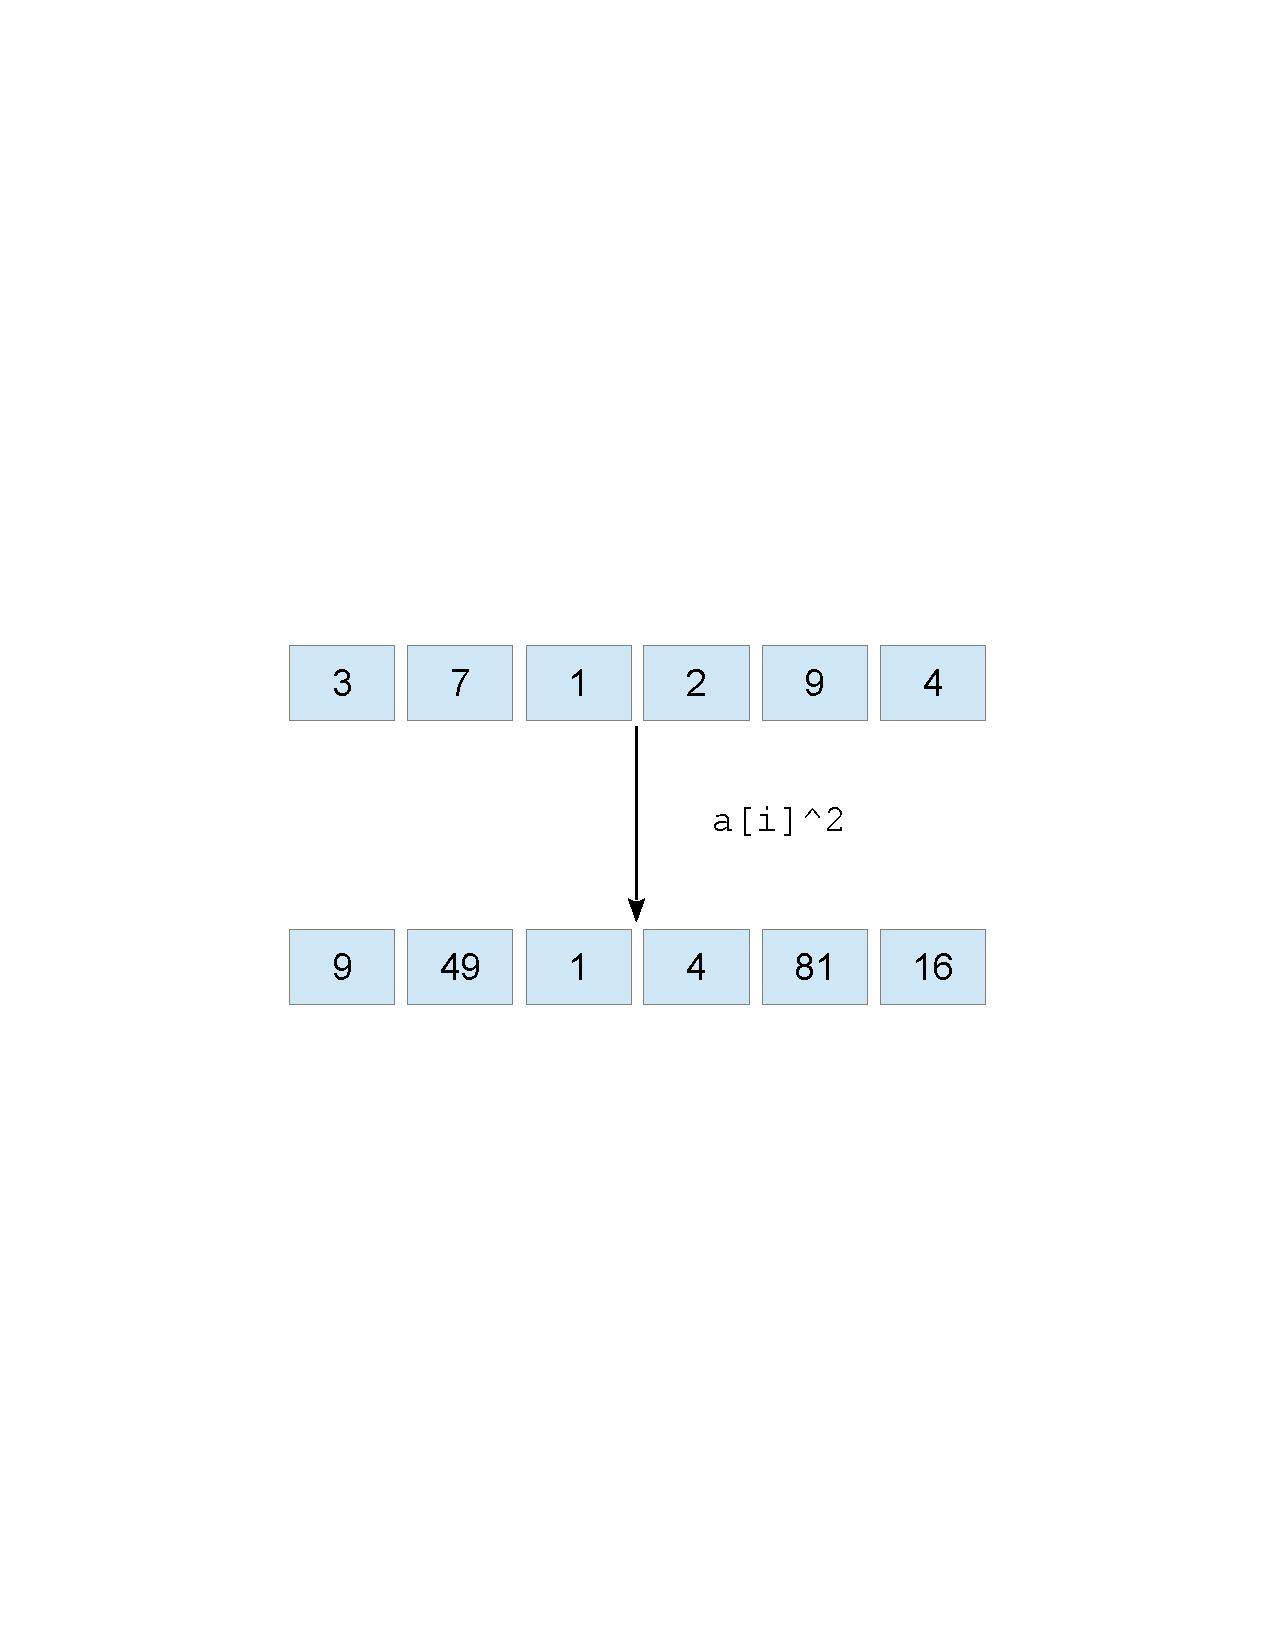
\includegraphics[scale=0.55, trim=4.5cm 10.5cm 4.5cm 10.5cm, clip]{ArraySquared.pdf}}
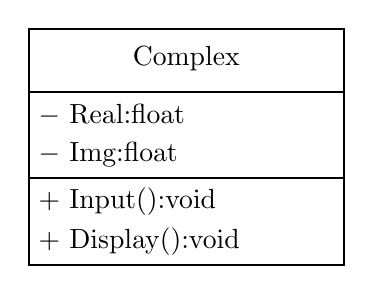
\begin{tikzpicture}
	% UML class box parameters.
	\def \displacementX {0.0cm}
	\def \displacementY {0.0cm}
	\def \DataY {1.1cm}	% No. of data members * 0.5cm + 0.1cm.
	\def \FunctionsY {1.1cm} % No. of functions * 0.5cm + 0.1cm.
	\def \SpanX {4cm}
	\def \CenterX {2cm}
	% Drawing class name box.
	\draw[thick] (\displacementX, \displacementY) rectangle (\displacementX+\SpanX, \displacementY-0.8cm);
	\coordinate [label=below:{\normalsize Complex}] (ComplexName) at (\displacementX+\CenterX,\displacementY-0.1cm);
	% Drawing data members box.
	\draw[thick] (\displacementX, \displacementY-0.8cm) rectangle (\displacementX+\SpanX, \displacementY-0.8cm-\DataY);
	\coordinate [label=right:$-$ Real:float] (Real) at (\displacementX,\displacementY-1.1cm);
	\coordinate [label=right:$-$ Img:float] (Img) at (\displacementX,\displacementY-1.1cm-0.5cm);
	% Drawing functions box.
	\draw[thick] (\displacementX, \displacementY-0.8cm-\DataY) rectangle (\displacementX+\SpanX, \displacementY-0.8cm-\DataY-\FunctionsY);
	\coordinate [label=right:$+$ Input():void] (Input) at (\displacementX,\displacementY-1.1cm-\DataY);
	\coordinate [label=right:$+$ Display():void] (Display) at (\displacementX,\displacementY-1.1cm-\DataY-0.5cm);
\end{tikzpicture}
\caption{UML Class Diagram}
\label{UML-Diagram-Complex-Class}
\end{figure}
\end{minipage}
\nocite{*}
\bibliographystyle{plain}
\bibliography{OOPref}
\end{document}
